\documentclass[usenames,dvipsnames,tikz]{standalone}
\usepackage{amsmath,amssymb}
\usepackage{xcolor}
\colorlet{tBlue}{RoyalBlue!35!Cerulean}
\colorlet{tRed}{Red}
\usepackage{tikz}
\usepackage{standalone}
\begin{document}
	
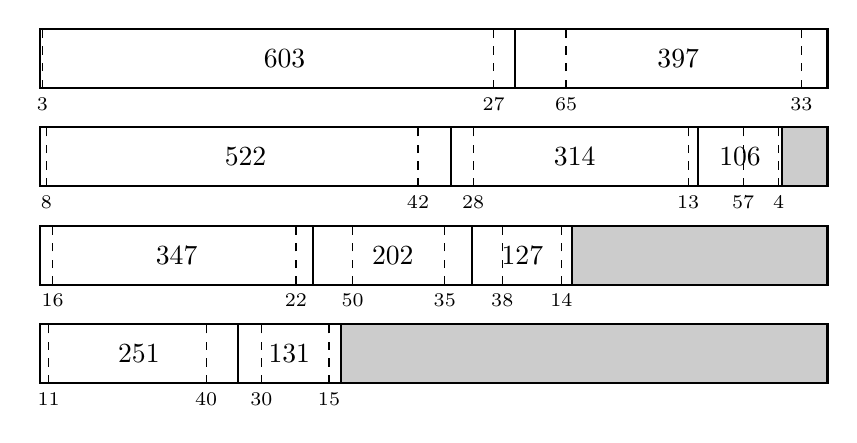
\begin{tikzpicture}
%\draw [help lines] (-1,-2) grid (12,5);
% 1=0.1, 2=0.15, 3=0.2, 4=0.25, 5=0.3
% 6 (3-27), 5 (8-42), 4 (33-65), 4 (16-22), 3 (13-28), 3 (11-40), 2 (35-50), 1 (15-30), 1 (14-38), 1 (4-57).

\draw [thick] (0,0) rectangle (10,0.75);
\draw [thick] (0,1.25) rectangle (10,2);
\draw [thick] (0,2.5) rectangle (10,3.25);
\draw [thick] (0,3.75) rectangle (10,4.5);

% Bottom row, 251, 131 (11-40, 30-15, sixth, tenth)
\draw [thick] (2.51,0) -- (2.51,0.75);
\draw [thick] (3.82,0) -- (3.82,0.75);
\filldraw[fill=black!20!white, draw=black, thick] (3.82,0) rectangle (10,0.75);

\draw [dashed] (0.11,0) -- (0.11,0.75);
\draw [dashed] (2.11,0) -- (2.11,0.75);
\node [below] at (0.11,0) {\scriptsize{11}};
\node [below] at (2.11,0) {\scriptsize{40}};

\draw [dashed] (2.81,0) -- (2.81,0.75);
\draw [dashed] (3.67,0) -- (3.67,0.75);
\node [below] at (2.81,0) {\scriptsize{30}};
\node [below] at (3.67,0) {\scriptsize{15}};

\node at (1.255,0.375) {251};
\node at (3.165,0.375) {131};

% Second from bottom row, 347, 202, 127 (16-22, 50-35, 38-14, fourth, seventh, ninth)
\draw [thick] (3.47,1.25) -- (3.47,2);
\draw [thick] (5.49,1.25) -- (5.49,2);
\draw [thick] (6.76,1.25) -- (6.76,2);
\filldraw[fill=black!20!white, draw=black, thick] (6.76,1.25) rectangle (10,2);

\draw [dashed] (0.16,1.25) -- (0.16,2);
\draw [dashed] (3.25,1.25) -- (3.25,2);
\node [below] at (0.16,1.25) {\scriptsize{16}};
\node [below] at (3.25,1.25) {\scriptsize{22}};

\draw [dashed] (3.97,1.25) -- (3.97,2);
\draw [dashed] (5.14,1.25) -- (5.14,2);
\node [below] at (3.97,1.25) {\scriptsize{50}};
\node [below] at (5.14,1.25) {\scriptsize{35}};

\draw [dashed] (5.87,1.25) -- (5.87,2);
\draw [dashed] (6.62,1.25) -- (6.62,2);
\node [below] at (5.87,1.25) {\scriptsize{38}};
\node [below] at (6.62,1.25) {\scriptsize{14}};

\node at (1.735,1.625) {347};
\node at (4.48,1.625) {202};
\node at (6.125,1.625) {127};

% Second from top row, 522, 314, 106 (8-42, 28-13, 57-4, second, fifth, eighth)
\draw [thick] (5.22,2.5) -- (5.22,3.25);
\draw [thick] (8.36,2.5) -- (8.36,3.25);
\draw [thick] (9.42,2.5) -- (9.42, 3.25);
\filldraw[fill=black!20!white, draw=black, thick] (9.42,2.5) rectangle (10,3.25);

\draw [dashed] (0.08,2.5) -- (0.08,3.25);
\draw [dashed] (4.8,2.5) -- (4.8,3.25);
\node [below] at (0.08,2.5) {\scriptsize{8}};
\node [below] at (4.8,2.5) {\scriptsize{42}};

\draw [dashed] (5.5,2.5) -- (5.5,3.25);
\draw [dashed] (8.23,2.5) -- (8.23,3.25);
\node [below] at (5.5,2.5) {\scriptsize{28}};
\node [below] at (8.23,2.5) {\scriptsize{13}};

\draw [dashed] (8.93,2.5) -- (8.93,3.25);
\draw [dashed] (9.38,2.5) -- (9.38,3.25);
\node [below] at (8.93,2.5) {\scriptsize{57}};
\node [below] at (9.38,2.5) {\scriptsize{4}};

\node at (2.61,2.875) {522};
\node at (6.79,2.875) {314};
\node at (8.89,2.875) {106};

% Top row, 603, 397 (3-27, 65-33, first, third)
\draw [thick] (6.03,3.75) -- (6.03,4.5);

\draw [dashed] (0.03,3.75) -- (0.03,4.5);
\draw [dashed] (5.76,3.75) -- (5.76,4.5);
\node [below] at (0.03,3.75) {\scriptsize{3}};
\node [below] at (5.76,3.75) {\scriptsize{27}};

\draw [dashed] (6.68,3.75) -- (6.68,4.5);
\draw [dashed] (9.67,3.75) -- (9.67,4.5);
\node [below] at (6.68,3.75) {\scriptsize{65}};
\node [below] at (9.67,3.75) {\scriptsize{33}};

\node at (3.105,4.125) {603};
\node at (8.105,4.125) {397};

\end{tikzpicture}

\end{document}